\documentclass[conference]{IEEEtran}
\IEEEoverridecommandlockouts
\usepackage{cite}
\usepackage{amsmath,amssymb,amsfonts}
\usepackage{algorithmic}
\usepackage{graphicx}
\usepackage{textcomp}
\usepackage{xcolor}
\def\BibTeX{{\rm B\kern-.05em{\sc i\kern-.025em b}\kern-.08em
    T\kern-.1667em\lower.7ex\hbox{E}\kern-.125emX}}
\begin{document}

\title{Effects of Fairness Constraints on Models of U.S. Federal Tax Policy}

\author{\IEEEauthorblockN{FSDN71}
\IEEEauthorblockA{\textit{Department of Computer Science} \\
\textit{University of Durham}\\
Durham, United Kingdom \\
fsdn71@durham.ac.uk}
}

\maketitle

\begin{abstract}
Income taxes are a mechanism by which governments raise revenue to fund spending programs and, to some extent, advance socio-economic fairness objectives through redistribution. However, tax policy is determined by complex human-devised logic, and even where specific policies are introduced with greater fairness intended, these can fail to achieve their specified objectives. We propose to first approximate the income tax prediction problem using publicly accessible survey microdata with deep neural networks, and then to apply fairness methods to the resulting function to induce fairness of post-tax outcomes across race and gender. We also present an analysis of the resulting changes to tax policy and its effects on the racial and gender groups in the survey.
\end{abstract}

\begin{IEEEkeywords}
Bias, AI, tax, neural network
\end{IEEEkeywords}

\section{Project Proposal}
The Annual Social and Economic Supplement (of the Current Population Survey) is a household survey of U.S. households with questions on financial circumstances, including questions on race, gender and other social variables. The microdata contains enough information on income sources and expenditure, as well as actual tax liabilities, to specify U.S. federal tax policy with reasonable accuracy. However, there is significant bias in post-tax incomes of individuals across racial and gender groups, with lesser incomes for nonwhite and female individuals, and more so for their intersections. Therefore, if there was a model predicting income tax liabilities (and therefore post-tax income), then the application of pre-processing, in-processing and post-processing fairness techniques could show how federal tax policy could reduce these disparities to avoid perpetuating them. 
\subsection{Motivation}
American federal tax policy raises over \$3tr annually, and is therefore a substantial part of the nation's finances. Its distributional impacts affect everyday households, and does not directly discriminate by race or gender. However, the role of the government transfers specified by the tax code does perpetuate existing biases in disposable income experienced by racial and gender groups by failing to account for the different distributions of taxable income. By comparing function approximations of tax policy before and after fairness methods are applied, we can demonstrate not just that there is a bias in post-tax incomes, but the degree to which an altered model of federal tax policy could reduce those biases, while still remaining reasonably accurate to existing tax liabilities.
\subsection{Research Tasks}
This project will involve a number of tasks to complete:
\begin{enumerate}
    \item Data collection: the ASEC microdata must have missing or invalid records removed, categorical features encoded in appropriate data types, and any other adjustments carried out. This will use Python libraries such as Pandas and NumPy.
    \item Data analysis: descriptive statistics will be used to explain the different patterns of the financial variables across racial and gender categories. Fairness metrics will be set based on the biases pre-existing in the data.
    \item Model development: architecture, training process and hyperparameters must be decided, and the model trained using supervised learning to approximate post-tax incomes indirectly by predicting federal tax liabilities. Metrics related to accuracy and impacts on sensitive attribute groups must be recorded. This will predominantly use TensorFlow for the model development, and Seaborn/Matplotlib/Plotly/Scikit-learn for data analysis.
    \item Fairness improvement: one fairness adjustment will be applied to the model, and all metrics recalculated.
    \item Analysis: the changes in accuracy and fairness metrics must be identified and contextualised.
\end{enumerate}
\subsection{Outcome}
The main outcome of this project will be an analysis of the trade-off in neural network-based tax policy modelling between accuracy to the current system, and fairness among racial and gender groups - whether fairness is relatively trivial to achieve without substantial tax overhaul, or whether the existing system is so efficient at perpetuating disparate impacts that fairness amendments would substantially change the current effects of its policies. This project will also produce an analysis of the existing bias of the tax system.

\section{Project Progress}
\subsection{Data Analysis}
\subsubsection{Data Cleaning}
The ASEC microdata contains a large number of columns, from which only 17 (excluding demographic variables) will be used as input features. These are mainly continuous variables, with binary variables for marital status (married/unmarried or separated) and tax filer status (joint/single). There is one non-binary categorical variable, for the individual's job industry if applicable. An important variable not used for prediction is the survey weight - the number of individuals that each record in the survey microdata represents, controlling for non-response and other biases. This is used in the calculation of all descriptive statistics, and will be used in the model training where possible, as this ensures that the survey has the highest possible similarity to the actual U.S. population. Categorical variables are converted to continuous variables by one-hot encoding - replacing a column with $k$ unique categories with $k-1$ columns, each indicating the presence of a different category in the original column. The last category is not necessary, as it is redundant by an all-zero row in the other columns. The dataset contains financial and age variables in their original form, so no bucketing is necessary. In addition to the above, the rows were removed where: the person is aged under 18, the person has no population weight, and the person paid less than \$50,000 in annual federal income tax. The restriction on income tax is due to significant uncertainty at the top of the income spectrum caused by survey bias\cite{RePEc:inq:inqwps:ecineq2017-452}. This affected $1.7\%$ of the dataset.
\subsubsection{Dataset Bias}
The dataset shows widespread and significant bias in both the financial variables, and in job industry. In job industries, men are more likely to work in business and construction, whereas women are more likely to work in education, health, hospitality, or not at all. Within these gender disparities, Asians are more likely to work in business, Black people in retail and White in manufacturing. Financial variables also show disparities - the racial group with the highest mean gross income the Asian group, followed by White, Black and Other (including mixed-race). Men also typically earn more than women. These disparities appear to stack on top of each other, with the mean gross income for Asian men over twice that of Black women, and around 230\% that of women with race `Other'. One interesting observation is the fact that while Asian men far outperform White men in rental income, the reverse is true for dividend income, perhaps suggesting a pattern of difference in the makeup of individual income for the two groups.
\subsubsection{Conventional Implementation}
The dataset was partitioned into training ($80\%$), validation ($10\%$) and testing ($10\%$) sets. Using the TensorFlow library\cite{tensorflow2015-whitepaper}, a selection of neural network architectures were defined and initialised with random weights. The first was a linear regression model, with the input $36$ features transformed into a one-dimensional feature from the weights and bias. The second was a fully-connected neural network with $16$ features after the first layer, $16$ after the second (both with ReLU\cite{2018arXiv180308375A} activation) and finally one feature with no activation function applied. The third was an altered version of the fully-connected network, in which half of the features in the first layer were activated with a sigmoid function - the motivation for this is the fact that tax legislation is broadly two sets of functions - functions which determine which side of a threshold a value is (returning Boolean values), and functions which apply rates to values (returning numerical values) - and therefore a combination of sigmoid and ReLU activations might enable closer function fitting. The models were trained for $256$ epochs using the optimizer Adam\cite{kingma2017adam} to minimise mean squared error and learning rate $0.001$. Figure 1 shows the validation losses achieved over time. Table 1 contains the deciles of mean absolute errors on the testing dataset, which indicate that for a large proportion of the dataset, the model was accurate within $\$500$, and overall loss was distorted by high-income cases.

The highest-performing model was found to be the ReLU-based neural network, which from this point is the only model considered. The model was additionally tested against unbiased versions of the dataset. With the advantage of having survey weights, we can resample the weights such that each race-gender combination has an equal population, with the total population remaining the same\footnote{For example, this involved multiplying the weights of `Asian-Female' records by $4.181$ and `White-Male' by $0.319$.}. This was done for both training and testing datasets.

\begin{figure}[h]
    \caption{Validation losses by epoch and model architecture}
    \centering
    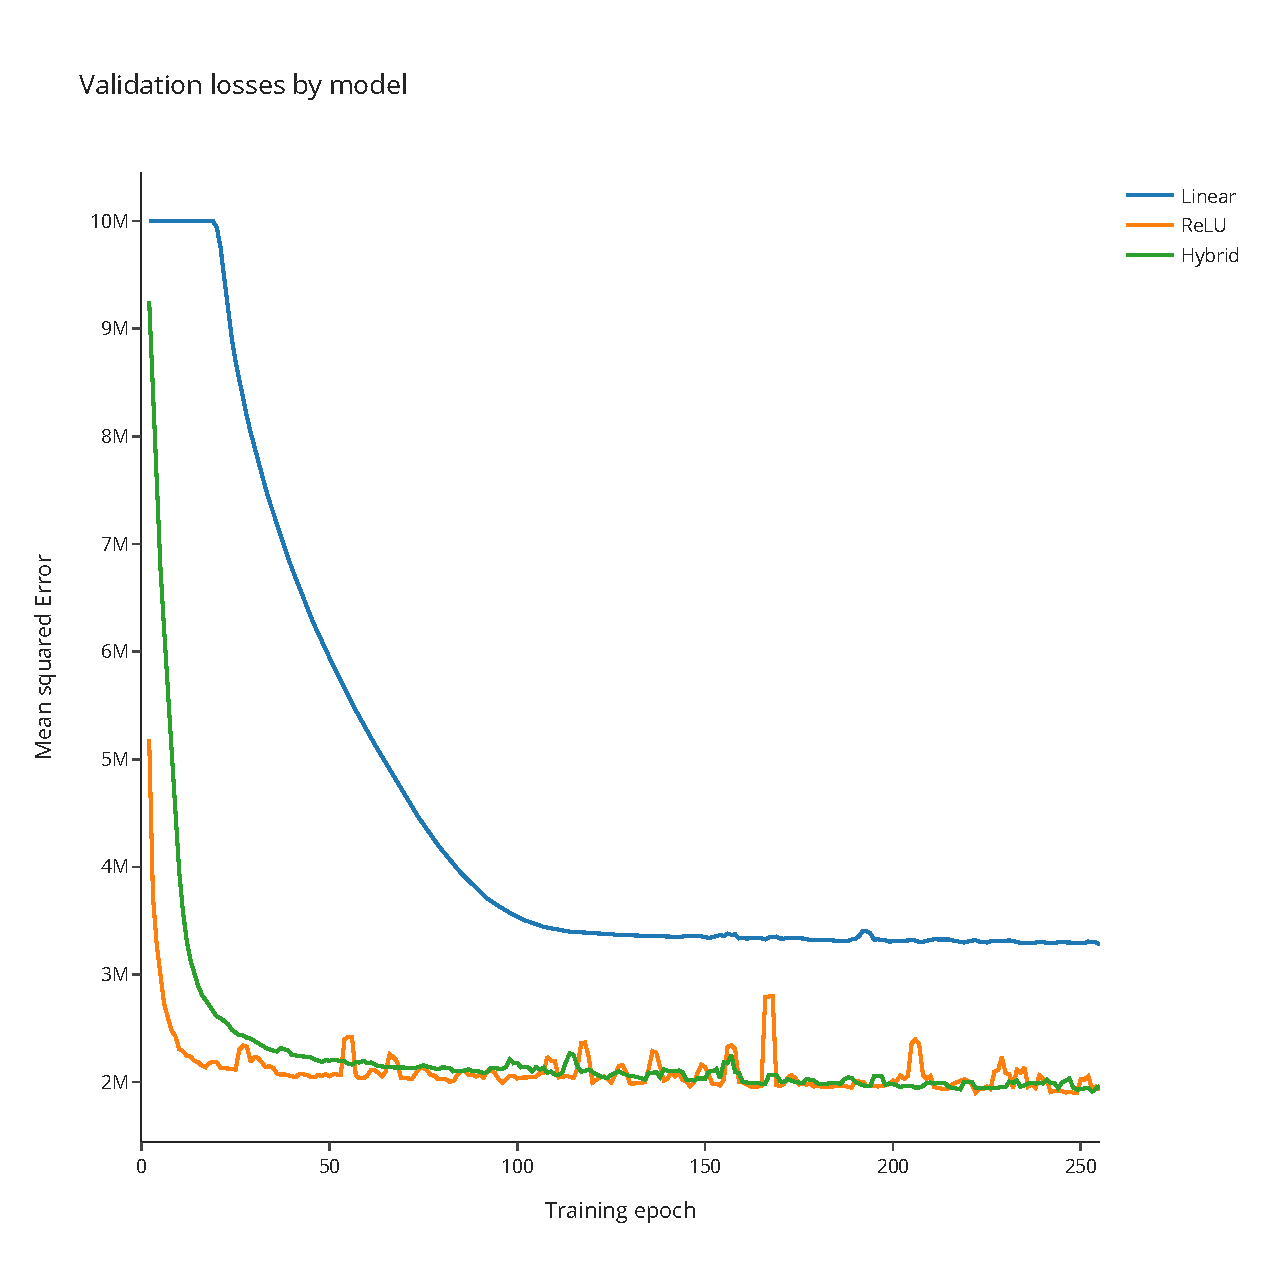
\includegraphics[width=0.5\textwidth]{figures/losses.eps}
\end{figure}

\begin{table}[]
    \caption{Mean absolute error deciles}
    \centering
    \begin{tabular}{llllllllll}
    Decile     & 1    & 2     & 3     & 4     & 5     & 6      & 7      & 8      & 9       \\
    Abs. Error & 6 & 16 & 28 & 51 & 89 & 187 & 345 & 594 & 1867
    \end{tabular}
\end{table}

\bibliographystyle{IEEEtran}
\bibliography{project_proposal}

\end{document}
